%\section{Design}
\section{Design and Implementation}
In this section, we describe the design of \tool{} by focusing on how our design
solves the challenges discussed in the previous section.

%\subsection{Overview}
%\subsection{Workflow}
\subsection{Design}
\tool{} has three steps,
as shown in Figure~\ref{fig:workflow}. First, we run the target program with a
concrete input (sensitive information) under the dynamic binary instrumentation
(DBI) frameworks to collect execution traces. After that, we run the symbolic
execution to capture the fine-grained semantic information of each
secret-dependent control-flow transfers and data-accesses. Finally, we run Monte
Carlo (MC) simulations to estimate the amount of leaked information.

\begin{figure*}[t]
    \centering
    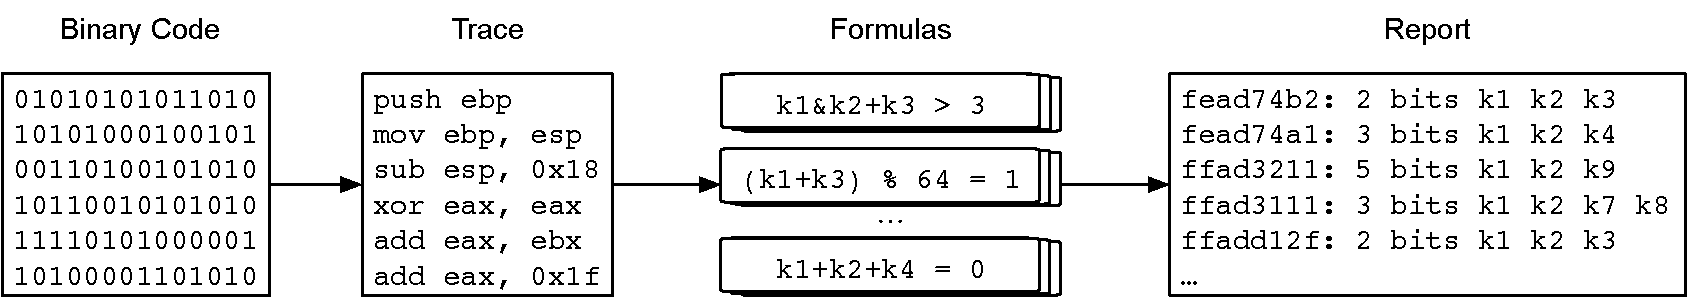
\includegraphics[width=0.8\textwidth]{./figures/workflow.pdf}
    \caption{The workflow of \tool{}.}
    \label{fig:workflow}
\end{figure*}

\begin{enumerate}
    \item \emph{Execution trace generation.} The design goal of \tool{} is to
          estimate the information leakage as precisely as possible. Therefore,
          we sacrifice the soundness for precision in terms of program
          analysis. We run the target binary under dynamic binary instrumentations (DBI) to
          to record execution traces and the runtime information.
          Once sensitive information is loaded into memory, we start to collect the 
          trace.
    \item \emph{Instruction level symbolic execution.} We model attackers'
          observations from side-channel vulnerabilities with logic formulas.
          Each formula captures the fined-grained information between input
          secrets and leakage sites. In consideration of precision and
          performance, we remove the intermediate language(IR) layer of the
          symbolic execution. Also, the engine only symbolically executes the
          instruction that might be affected by the input key. We use random
          testing instead of SMT solvers to find satisfying variables. 
    \item \emph{Leakage estimation.} We transfer the information leakage quantification
          problem into the problem of counting the number of assignments that satisfy the
          formulas which model the observations from attackers. We propose a
          Monte Carlo method to estimate the number of satisfying solutions.
          With the help of the Central Limit Theorem (CLT),
          we also give an error estimate with the probability,
          which gives us the \emph{precision guarantee}.

\end{enumerate}


%% \subsection{Trace Logging}
%% The trace information can be logged via some emulators (e.g., QEMU) or 
%% dynamic binary instrumentation tools (DBI). 
%% We run a program with the concrete input under the DBI to record
%% execution traces.
%% The trace data has the following information:
%% \begin{itemize}
%%     \item Each instruction mnemonics and its memory address.
%%     \item The operands of each instruction and their concrete values during the 
%%           runtime.
%%     \item The value of EFLAGS register. 
%%     \item The memory address and the length of the sensitive information.
%%      Most crypto libraries stores sensitive information in arrays,
%%      variables or contiguous buffer.
%% \end{itemize}

%% \subsection{Instruction Level Symbolic Execution}
%% \label{InstructionSE}
%% The primary purpose of the step is to generate constraints of the input 
%% sensitive information from the execution trace. 
%% If we give the target program a new input which 
%% is different from the original input that was used 
%% to generate the execution trace but still satisfies those constraints,
%% as an attacker, he will have the same observations on
%% control-flow transfer and 
%% data-access patterns.

%% The tool runs symbolic execution on top of execution traces.
%% At the beginning of the symbolic execution, the tool creates new 
%% symbols for each byte in the raw buffer. For other data in the 
%% register or memory at the beginning, we use actual values from the 
%% runtime information collected during the runtime. 
%% During the symbolic execution for each instruction, 
%% the tool updates every variable in the memory and registers with a
%% math formula. The formula is made up of concrete values and the input 
%% key as the symbols accumulated through the symbolic execution.
%% For each formula, the tool will check weather it can be reduced
%% into a concrete values (e.g., $k_1+12-k_1 = 12$ ). 
%% If so, the tool will only use the concrete values in the 
%% following symbolic execution.

%% \subsubsection{Verification and Optimization}
%% We run the symbolic execution (SE) on top of x86 instructions.
%% In other words, we do not rely on any intermediate languages to simplify the implementation of symbolic execution. 
%% While the implementation itself has a lot of benefits (Better performance, accurate memory model), 
%% we need to implement the symbolic execution rules for each x86 instruction. 
%% However, due to the complexity of x86, it is inevitable to make mistakes. 
%% Therefore, we verify the correctness of the SE engine during the execution. 
%% The tool will collect the runtime information (Register values, 
%% memory values) and compare them with the formula generated from the symbolic execution. Whenever the tool finishes the symbolic execution of each instruction, the tool will compare the formula for each symbol and its actual value. If the two values do not match, we check the code
%% and fix the error. Also, if the formula does not contain any symbols,
%% the tool will use the concrete value instead of symbolic execution.

%% \subsubsection{Secret-dependent control-flows}
%% An adversary can infer sensitive information from secret dependent control-flows. 
%% There are two kinds of control-transfer instructions: the unconditional 
%% control-transfer instructions and the conditional transfer instructions.
%% The unconditional instructions, like CALL, JUMP, RET transfer control
%% from one code segment location to another. Since the transfer is independent of the input sensitive information, an attacker was not able to infer any sensitive information from the control-flow. 
%% So the unconditional control-transfer does not leak any information based on our threat model. During the symbolic execution, 
%% we update the register information and memory cells with new formulas accordingly.

%% The conditional control-flow transfer instructions, like conditional jumps,
%% depending on CPU states, may or may not transfer control flows.
%% For conditional jumps, the CPU will test if certain condition flag 
%% (e.g., CF = 0, ZF =1) is met and jump to certain branches, respectively.
%% The symbolic engine will compute the flag and represent the flag in a symbol 
%% formula. Because we are running on a symbolic execution on an execution trace, 
%% we know which branch is executed.
%% If a conditional jump uses the CPU status flag, we will generate the constraint 
%% accordingly.


%% %\begin{figure}[ht]
%% %      \centering
%% %      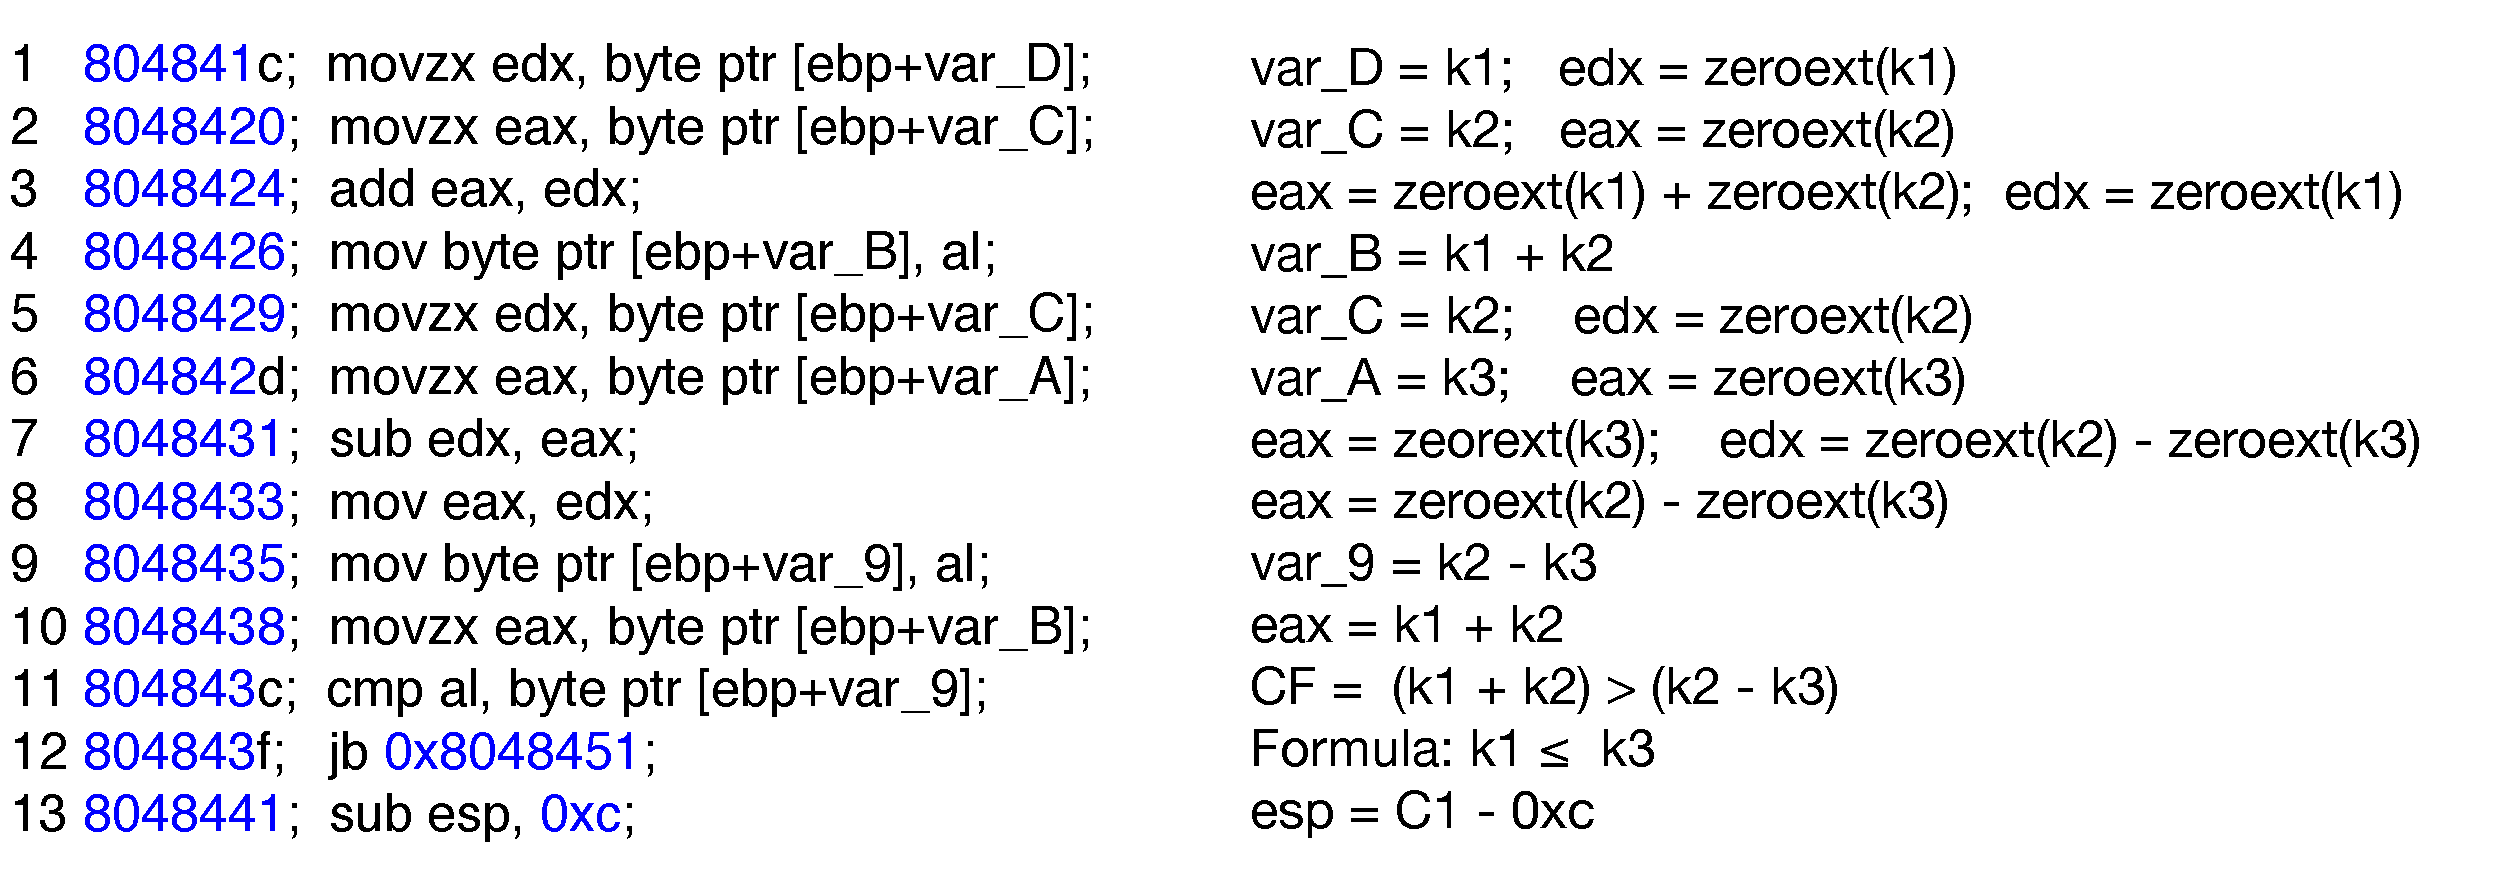
\includegraphics[width=\columnwidth]{./figures/secretCF.pdf}
%% %      \caption{The workflow of \tool{}. \fixme{fix the caption, fix the drawing.} \fixme{duplicate label.}}
%% %      \label{fig:Test-------------------}
%% %  \end{figure}

%% For examples,

%% \begin{lstlisting}
%% ...
%% 0x0000e781      add dword [local_14h], 1
%% 0x0000e785      cmp dword [local_14h], 4
%% 0x0000e789      jne 0xe7df
%% 0x0000e78b      mov dword [local_14h], 0
%% ...
%% \end{lstlisting}

%% At the beginning of the instruction segment, the value at the 
%% address of local\_14h can be written as $F(\vec{K})$. At the address $e785$, 
%% the value will be updated with $F(\vec{K})+1$. Then the code compares 
%% the value with 4 and use the result as a conditional jump. 
%% Based on the result, we can have the following formula:

%% $$F(\vec{K}) + 1 = 4$$

%% The formula, together with the memory address (0xe789) is store
%% as a \textit{formula tuple (address, formula)}. 
%% Each formula tuple represents one leakage site.

%% \subsubsection{Secret-dependent data access}
%% Like input-dependent control-flow transfers, an adversary can also infer 
%% sensitive information from the data access pattern as well. 
%% We try to find this kind of leakages by checking 
%% every memory operand of the instruction. We generate the memory addressing 
%% formulas. As discussed before, every symbols in the formula is the input key. 
%% If the formula does not contain any symbols, the memory access is independent 
%% from the input sensitive information and will not leak any sensitive information 
%% according to our threat model. Otherwise, we will generate the constraint for
%% the memory addressing. We model the memory address with a symbolic formula 
%% $F(\vec{K})$. 
%% Because we also have the concrete value of the memory address $Addr1$. 
%% Inspired by the work from~\cite{203878}, the formula can be written as:
%% $F(\vec{K}) >> L = Addr1 >> L$

%% $L$ represents the minimum memory address granularity that an attacker 
%% can observe. For example, Flush and Reload can distinguish between different
%% cache lines, which means the value of L is 6.

%% \subsubsection{Information Flow Check}
%% \tool{} is designed to help software developers find and understand the 
%% side-channel vulnerabilities. To ease the procedure of fixing the bug,
%% we also track the information flow for each byte of the input
%% buffer. 
%% The step can be seen as the multiple-tag taint analysis.
%% With the help of the information from symbolic execution, we can implement 
%% a relatively simple but relatively precise information flow track.
%% At the beginning of the analysis, \tool{} keep a track for each byte in 
%% the original buffer. When \tool{} symbolically executes each
%% instruction in the trace, it will check every value read from
%% registers or memory. If the value is concrete, it means the
%% instruction has nothing to do with the original buffer.
%% If the value is a formula, it means the original information passes through 
%% the instruction. Since each byte in the sensitive
%% buffer is represented as a symbol with a unique ID, \tool{} can
%% know which byte in the origin buffer goes through the
%% instruction.


